\chapter{Testing}

The project requirements state \textit{"Given the target audience, the system should be robust and difficult to crash."} In order to achieve this, testing should be a priority to ensure a functional system. Furthermore, the testing of this project (as proven below) is comprehensive and attempts to cover all eventualities. With a combination of automated, manual and user testing, a reasonable degree of confidence can be stated with regards to the robustness of both the hologram and charades systems. 

Whilst data security did not need to be considered for this project (as no sensitive data is stored) security against cyber attacks and malicious use have been considered throughout the testing and development process. For the most part, manual testing has been used to uncover potential flaws in the security of the website and, when discovered, additional automated tests have been added to safeguard against these issues in the future.

\section{Overall Approach to Testing}
The project used TDD as part of the process for software implementation. As well as designing features, tests were also designed for the required functions before any implementation. There were two main types of tests for the website: unit tests, which test the functionality of the model and controllers, and system tests, which use Selenium to check the flow of the system and simulate the actions of a user. Where appropriate, tests for functions were designed to test three different cases:

\begin{itemize}
\item Success case: Simulates either an expected input parameter for the function or an expected state that the system should be in to run a function.

\item Edge case: Checks the maximum range of the functions input parameters. For example, if the function was only designed to allow 5 viewers to participate in a game, then the test case would check that the when the viewers total 5 the function still passes.

\item Failure case: Ensures that given incorrect parameters or system state, the function will fail in the expected way.

\end{itemize}

An example function and corresponding test cases displaying the above approach to testing can be found in Appendix C, section \textit{Unit test}.

Unit tests were organised into classes where each test class would exercise a single class or module of code. Similarly, system tests were designed to test a single Django template. All test classes are held in test files prefixed with \textit{test\_} and these can be found in the \textit{python/tests} and \textit{charades/charades/test} directories. The requirement for adding code to the master branch is that all unit and system tests (past and present) must pass, and the static analysis tools must produce no errors.


\section{Automated Testing}
\subsection{Jenkins}
To improve the consistency of the code base, the GitHub repository was linked to a local Jenkins server. This server was set up at the beginning of the project and was used as part of the development life cycle of each feature. The Jenkins server ran as a background process on the development machine. The set up for the Jenkins server followed two guides: The official Jenkins Windows Service installation guide \textit{"Installing Jenkins as a Windows Service"} \cite{jenkins_wiki_install} from the Jenkins.io wiki and Steve's Blog \textit{"Automated python unit testing, code coverage and code quality analysis with Jenkins"} \cite{steves_blog}, a self hosted technical blog from a software development consultant specialising in Python.

Whilst Jenkins offers the ability to run tests periodically, this feature was not used and tests were triggered manually by the developer. The reasoning behind this is that time based builds were not required. Had the project been developed by a team, the need for timed builds is more justifiable as many developers will be pushing code changes simultaneously. In a single person developer team, code is pushed one feature at a time and the work flow is linear, hence there is no justifiable requirement for periodic builds. Despite this, the use of Jenkins is still valid in a single developer project, as it allows for centralised building of the project in a controlled, repeatable, environment. Additionally, the formatting of results produced by Jenkins offers an easy way to quickly identify problems within the code base.

\subsection{Static analysis}
\subsubsection{Pylint}
Pylint is a linting tool that follows the PEP8 standards \cite{pep8} for Python coding. The linter runs static analysis on the code base and ensures that all code meets with the standards specified by PEP8 (and produces warning and errors were this is not the case). The PEP8 standards include guidelines for style and syntax, as well as documentation (in the form of doc strings). Whilst several alternative standards for the Python coding language are available, PEP8 was chosen as it is promoted by the developers of the Python language and is the most popular amongst the community. An example of the Pylint output rendered by Jenkins is displayed in Figure \ref{fig:jenkins_pylint}. In this Figure, the peaks correspond to when pull requests are initially pushed to Jenkins and troughs are were the Pylint warnings have been resolved.
\begin{figure}[h!]
	\centering{
		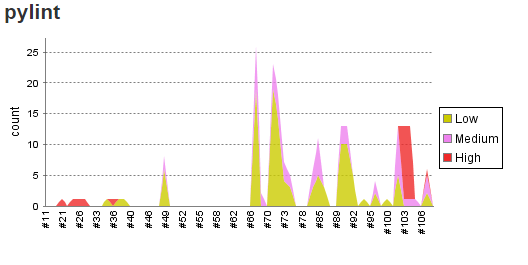
\includegraphics[scale=0.75]{Chapter4/jenkins_pylint.PNG}
		\caption{The output of the Pylint test run on the full code base rendered by Jenkins. Here, the number of warnings, and their severity, is logged by each build number.}
		\label{fig:jenkins_pylint}
	}
\end{figure}

\newpage

\subsubsection{Test coverage} 
An additional testing package, nosetest \cite{nosetest}, was used to run Python tests for this project. This package produces reports that are interpretable by Jenkins for both unit tests and test coverage. The test coverage displays graphically the proportion of the code that is run in tests. Although basic, this helps to highlight potential conditional statements, function and even lines that are not being tested. As the web based charades game was written in Django (which has its own testing framework), nosetest could only be used for the hologram creation software.

An example of the test coverage output rendered by Jenkins is displayed below in Figure \ref{fig:jenkins_test_cover}. It shows that whilst the majority of the code base is covered by testing, several lines are excluded. These lines had to be omitted from tests as their functionality was to perform the video processing loop. Whilst the functions that are called within the loop are sufficiently tested, the loop itself can not be tested easily as it creates an output window. The output window is only successfully closed via mouse click on the window close button (an operation that is not easily replicated within unit tests).
\begin{figure}[h!]
	\centering{
		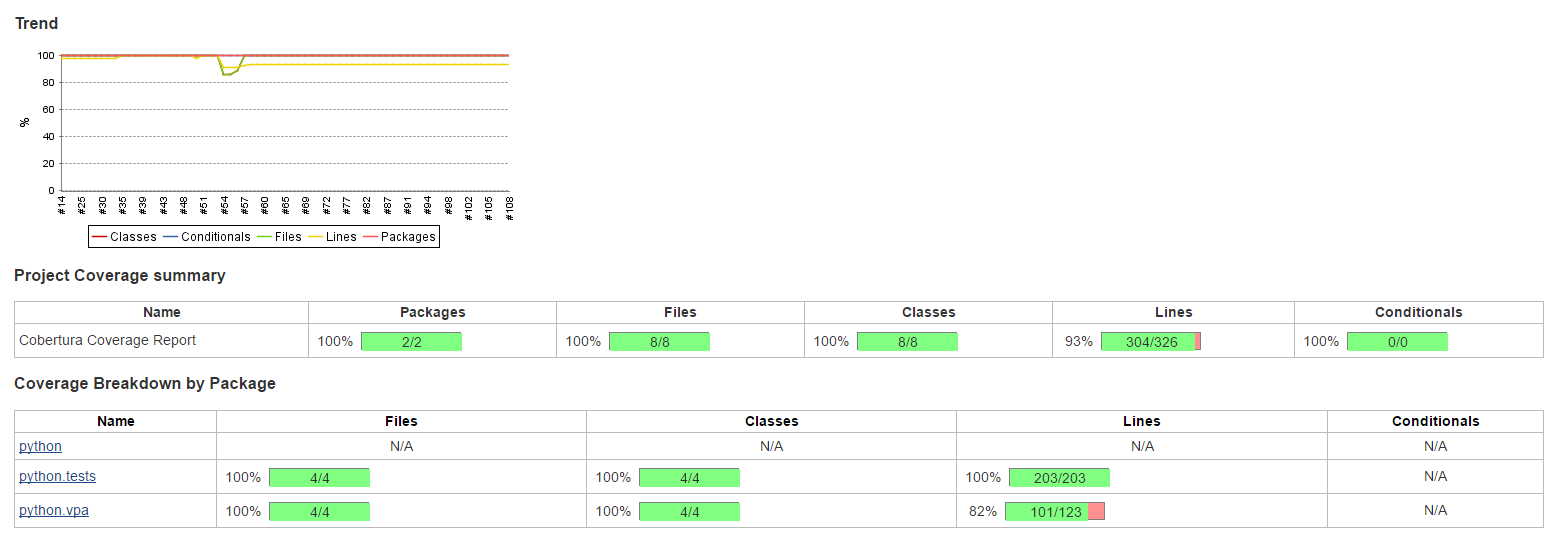
\includegraphics[scale=0.75]{Chapter4/jenkins_test_coverage.PNG}
		\caption{The rendered output of the test coverage report from nosetest in Jenkins. Note the incomplete test coverage for Lines (yellow) and see explanation in section 4.2.2.2.}
		\label{fig:jenkins_test_cover}
	}
\end{figure}
 

\subsection{Unit Tests}
To ensure the functionality of the system, unit tests were created to test functions. The unit tests were written using the Python unit test framework provided by the Python language \cite{python_unittest}. The unit tests are designed to be atomic and test a single part of functionality per test. As such, more complex functions that are dependant on the state of the system, or have multiple return values, will have multiple tests associated with them, designed to exercise every line of the code. Unit tests were written in classes where one class will test only one Python class or module.

The tests for the hologram creation software are stored in a different directory to the source code, meaning the functions can not be directly called from the unit tests. Python's solution to this is to import the source code modules from the other directory using the keyword
\begin{verbatim}
import
\end{verbatim}
This, however, is only possible if the shared parent directory of both the tests and source code is a Python module itself. If this is not the case, a context file should be used to resolve the issue. The context file (Appendix C, section \textit{Context file}) is used to import the module by first setting the correct directory path for Python to be able to find it, then importing the module from the current working directory. The context file is then imported at the start of every test.

Figure \ref{fig:jenkins_unit_test} shows the graph created by Jenkins and nosetest that represents the pass and failure state of each unit test for every build. The graph shows an upwards tread as the number of tests being created in the project increase with the creation of additional features. To be accepted into the master branch of the GitHub repository, all tests must pass.

\begin{figure}[h!]
	\centering{
		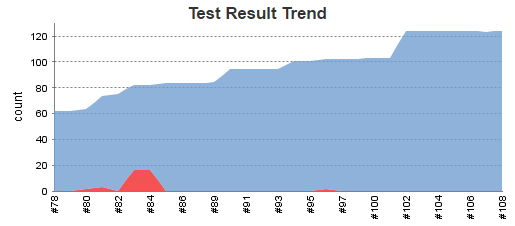
\includegraphics[scale=0.75]{Chapter4/jenkins_unit_test.PNG}
		\caption{The rendered output of the unit test report in Jenkins. Blue indicates tests which pass, while red indicates those which failed.}
		\label{fig:jenkins_unit_test}
	}
\end{figure}

\subsection{User Interface Testing}
The Python Selenium module was used for all tests of the user interface. The Selenium library allows for interaction with a web browser in a testing environment. By providing a URL for a website, Selenium will load that web page and then allows common user input actions to be performed programmatically. These actions include, but are not limited to, button clicks, filling in text fields and changing the current URL of the page. All user interface tests, for this project, have several generic test cases are always implemented. These are:

\begin{itemize}
	\item Page elements: The generic view of a page is tested to ensure that the elements on the page are what the test expects. This is mainly used as a test of the Django template code, written in HTML, and the embedded Python.
	\item Navigation: Most pages of the website will either have a button to take the user to another page, or poll the API until the conditions are met to redirect the user. In both cases, a test case will exist to ensure the page transition is correct. 
\end{itemize}

In addition to these tests, the website had to be tested to ensure that the URL could not be manually changed to affect the state of the game. An example of this would be attempting to visit the phrase\_selection.html page (where the actor selects a phrase) as a viewer.  In a scenario like this, the viewer is redirected to the index page with an error message displayed.

\subsubsection{Selenium start up time}
For continuity between tests, much of the online documentation that was used in this project, such as \textit{"Selenium with Python : Using Selenium to write tests"} \cite{selenium_guide}, proposed running a new instance of the Selenium web browser for each test. The reason for doing this is that it will restart the web browser and remove any cached data or session information. When run locally on the developer machine, Selenium took on average 6 to 8 seconds to create a new instance of a web browser. Hence, with a growing number of Selenium test, the time taken to run the full test suite was no longer practical.

To remedy this, the decision was made to use only one Selenium web browser instance per class of tests \cite{django_live_server_test}. The Selenium instance was initialised in the class setUp function and closed in the class tearDown, and then the cached data was manually removed from the web browser instance. Whilst this does leave scope for having some cached data remain in the web browser between tests, this reduced the number of web browser reinitialisations to be equate to the number of test classes (8) as opposed to the number of test cases (27), hence saving over a third of the time when executing the tests.

\subsubsection{Using Selenium with Django and Localhost}
During the development of the project, the website was hosted on the local development machine using local host. In order to test the website with Selenium, a hosted version of the website must be accessible. For manual developer testing, Django offers the ability to run a server locally and host the website using the command: \begin{verbatim}
python manage.py runserver 
\end{verbatim}
to start the server. The website is then accessible from http://localhost:8000 (by default). To allow Selenium tests to run successfully, a method of starting the server before tests were run, needed to be implemented.

A possible way of doing this was to run the above command to start the server before tests were run. Whilst this does resolve the problem, it forces the tests to be reliant on the correct port (default 8000) being used to access the website. This port can be specified upon starting the server, but this could produce conflicts in different development environments if, for example, the development machine had other services running on the same localhost  port.

A more permanent solution was discovered in the Django documentation \cite{django_live_server_test}. This section of the documentation described the use of extending the StaticLiveServerTestCase rather than extending Python UnitTest. The extra functionality provided by extending this module means that when the test class is run, it launches a live Django server to host the Django web content stored in the same project. This service defaults to running on http://localhost:8081, but the full URL is accessible during test execution with the Python code:
\begin{verbatim}
self.live_server_url
\end{verbatim}
This above code returns a string value that matches the correct port address on localhost. Using the LiveServerTestCase resolves both problems mentioned above as firstly, there is no longer a need to hard code the URL for the localhost server address and secondly, the server exists only for the life span of the test meaning there is no need to start a separate server manually before the tests are executed.

\section{Manual Testing}
\subsection{Charades Game}
In addition to testing the web site code with automated unit tests, during most features, a manual test performed by the developer was carried out. Manual testing was designed to be a supplementary testing phase to ensure that functionality was correct and no exceptions or errors were raised unexpectedly. In the case that problems were discovered, these issues would be written as a formal test case and added to the test classes to ensure the functionality is checked in the future. The Manual testing followed multiple patterns of use.
\begin{itemize}
	\item Normal user work flow: The expected user work flow is followed to ensure that a typical user performing valid, and expected, operations causes the expected behaviour of the system with no failures.
	
	\item Unexpected behaviour: Users will not always follow the expected work flow of the website and can occasionally enter values incorrectly. This testing was performed on new features user interfaces and ensured:
	\begin{itemize}
		\item No invalid entries could be put into text or number entry fields.
		\item Submitting blank fields in forms does not produce errors. 
		\item Pressing the back button on a web browser does not cause errors for either the user or the system.
	\end{itemize}
	
	\item Malicious behaviour: Tests were carried out to ensure that the website could not be compromised deliberately by a user. Some of the information passing in this website uses the HTTP GET protocol and subsequently, that information is stored in the client side URL. It is possible that a user with malicious intentions may attempt to taint the information provided in the URL to corrupt the system. As such, tests were carried out to ensure that information in the URL was sanitised and expected.
\end{itemize}


\subsection{Hologram creation software}
Manual testing was carried out on a smaller scale for the hologram creation program. As discussed in section 4.2.2.2, several lines of code within the main display loop could not be unit tested. To ensure the functionality of this code, manual testing was performed to ensure correct functionality. This was the only manual testing performed on the hologram creation program as there was no user input and output required.


\section{User Testing}
User testing took place at the Aberystwyth Science week event in March 2017. The event lasted for three days and gave the opportunity to test the prototype of the hologram system with the target audience. A black tent was set up in the event hall and this housed the touch screen table being used as an external monitor for the holographic display. The web cam for the video feed input was set up outside the tent and used to record viewers. When new viewers entered the viewing area, initially a test video would be running and then, after explaining the technique, audience members were given the opportunity to be filmed to create a hologram that was displayed to their peers.

\subsection{General findings}
The stall at the event generated much intrigue amongst the audience. Many thoroughly enjoyed seeing their peers projected holographically, but there was a clear lack of purpose for those being filmed other than waving to a camera. This helped to confirm the need for the charades system to be used alongside the hologram creation system.

\subsection{Limited time}
Given the events size, the number of stalls and the limited time that each visiting school had at the event, a new consideration needed to be made regarding the amount of time required to play the game. Whilst the initial idea had been to swap users who were acting after every correct guess, this would invest a lot of the time that users had at the stall with swapping players rather than playing the game. To accommodate for this, the game flow was amended to have 3 phrases acted by the same actor and points accumulated by the viewers.

\subsection{Camera distance}
The charades game will require the actors whole body to be visible on camera while they are acting. At the event only the head of the actor was filmed using a standard web cam. Whilst this was in part because there was no advantage to filming the rest of the body given the state of the prototype, this was affected by the amount of space in the event hall. To resolve this issue at the next event, a wide angle camera orientated vertically would allow for a larger amount of the body to be filmed in same amount of space. However, this approach may require adaptations of the hologram creation software to avoid over cropping the video feed.